\documentclass[12pt,a4paper]{article}
\usepackage{indentfirst}
\usepackage[utf8x]{inputenc}
\usepackage{ucs}
\usepackage[MeX]{polski}
\usepackage{fancyhdr}
\usepackage{amsmath}
\usepackage{amsfonts}
\usepackage{amssymb}
\usepackage{subfig}
%\usepackage{supertabular}
\usepackage{array}
\usepackage{tabularx}
\usepackage{hhline}
\usepackage{tabulary, booktabs}
\usepackage{float}
\usepackage{lscape}
\usepackage[table]{xcolor}
\pagestyle{fancy}
\usepackage{graphicx}
\usepackage{multirow}
\newenvironment{bottompar}{\par\vspace*{\fill}}{\clearpage}
 
\begin{document}
\clearpage
\thispagestyle{empty}
 
\begin{figure}[H]
\centering

\includegraphics[scale=1.3]{logo.png}
\end{figure}
 
\vspace{16pt}
 
\begin{center}
\textbf{\huge Bazy Danych (Projekt)}
 
\vspace{30pt}
 
\textbf{\LARGE Analiza danych pogodowych}
 
 
\vspace{22pt}
 
\LARGE Opis projektu
 
\end{center}
 
\vspace{20pt}
 
\flushleft Autorzy: Dymitr Choroszczak 218627, Krzysztof Dąbek 218549\\
Kurs: Bazy danych (projekt)\\
Temat: Analiza danych\\
Prowadzący: dr hab. inż. Grzegorz Mzyk, prof. PWr\\
Termin zajęć: piątek 9:15\\
 
 
\newpage
 
\tableofcontents
 
\newpage
 
\section{Opis projektu}
 
\subsection{Koncept projektu}
\normalsize
Projekt jest realizowany w ramach kursu Bazy Danych na specjalności Robotyka (ARR), na kierunku Automatyka i Robotyka (AiR), na wydziale Elektroniki (EKA), na Politechnice Wrocławskiej.\\
Celem projektu jest stworzenie bazy danych przechowującej informacje pogodowe z różnych stacji, pobierane z serwera oraz zaimplementowanie metod analizy danych i wizualizacji wyników.\\
Dane do analizy zostaną pobrane z serwera ogimet.com dla wielu stacji pogodowych w Polsce i zapisane w tabelach.\\
Standardowy użytkownik bazy ma uprawnienia jedynie do wyświetlania wyników analizy oraz danych pogodowych.\\
Administrator ma dodatkowo możliwość dodawania, usuwania i zmiany stacji pogodowych, dla których będą pobierane dane.\\
Wynikiem analizy danych są wykresy zależności różnych czynników pogodowych od siebie, wykresy porównawcze dla różnych stacji pogodowych oraz automatycznie generowany komentarz dotyczący warunków w pobliżu danej stacji.
 
\subsection{Tabele}

\begin{itemize}
\small
\item Stacje pogodowe (Stations id)
    \begin{itemize}
	\item Stacja pogodowa (MeteoStation id)
	\item Położenie (Localization id)
    \item Automatyczny komentarz
    \item Komentarz analityka
    \end{itemize}
\item Stacja pogodowa (MeteoStation id)
    \begin{itemize}
    \item Data
    \item Godzina
    \item Temperatury (Temperatures id)
    \item Wilgotność
    \item Wiatr (Wind id)
    \item Ciśnienie
    \item Opady
    \item Zachmurzenie (Clouds id)
    \item Widoczność
    \end{itemize}
\item Położenie (Localization id)
	\begin{itemize}
	\item Stacje pogodowe (Stations id)
	\item Szerokość geograficzna
    \item Długość geograficzna
    \item Wysokość (m n.p.m.)
	\end{itemize}
\item Temperatury (Temperatures id)
    \begin{itemize}
    \item Stacja pogodowa (MeteoStation id)
    \item minimalna
    \item średnia
    \item maksymalna
    \end{itemize}
\item Wiatr (Wind id)
    \begin{itemize}
    \item Stacja pogodowa (MeteoStation id)
    \item kierunek
    \item prędkość
    \item porywy
    \end{itemize}
\item Zachmurzenie (Clouds id)
	\begin{itemize}
	\item Wskaźnik całkowity
	\item Wskaźnik dolny
	\end{itemize}
\item Administratorzy (Admin id)
    \begin{itemize}
    \item Login
    \item Hasło
    \item Imię
    \item Nazwisko
    \item e-mail
    \end{itemize}
\item Analitycy (Analyst id)
    \begin{itemize}
    \item Login
    \item Hasło
    \item Imię
    \item Nazwisko
    \item e-mail
    \end{itemize}
\end{itemize}
 
\subsection{Zależności}
%graf z kluczykami i dziwnymi strzalkami
 
\subsection{Lista funkcjonalności}
%tabelka z rolami uzytkownikow

\begin{figure}[!htb]
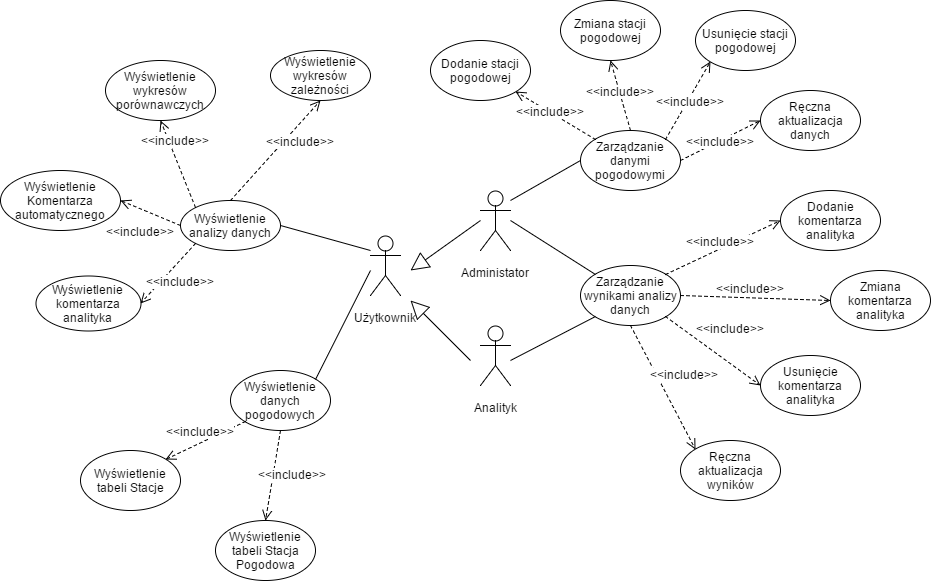
\includegraphics[width=\textwidth]{./figures/DiagramPrzypadkowUzycia.png}
\caption{Diagram przypadków użycia}
\end{figure}
 
\begin{enumerate}
\item Użytkownik
    \begin{itemize}
    \item Wyświetlenie analizy danych
        \begin{itemize}
        \item Wykresy zależności czynników pogodowych
        \item Wykresy porównawcze warunków między stacjami
        \item Komentarz automatyczny
        \item Komentarz analityka
        \end{itemize}
    \item Wyświetlenie danych pogodowych
        \begin{itemize}
        \item Wyświetlenie tabeli Stacje
        \item Wyświetlenie tabel Stacja Pogodowa
        \end{itemize}
    \end{itemize}
\item Administrator (dziedziczy po użytkowniku)
    \begin{itemize}
    \item Zarządzanie danymi pogodowymi
        \begin{itemize}
        \item Dodanie stacji pogodowej
        \item Usunięcie stacji pogodowej
        \item Zmiana stacji pogodowej
        \item Ręczna aktualizacja danych
        \end{itemize}
    \item Zarządzanie wynikami analizy danych
        \begin{itemize}
        \item Zmiana komentarza analityka
        \item Ręczna aktualizacja wyników
        \end{itemize}
    \end{itemize}
\item Analityk (dziedziczy po użytkowniku)
    \begin{itemize}
    \item Zarządzanie wynikami analizy danych
        \begin{itemize}
        \item Zmiana komentarza analityka
        \item Ręczna aktualizacja wyników
        \end{itemize}
    \end{itemize}
\end{enumerate}
 
\end{document}